%%%%%%%%%%%%%%%%%%%%%%%%%%%%%%%%%%%%%%%%%%%%%%%%%%%%%%%%%%%%%%%%%%%%%%%%%%%%%%%%
% Thesis / Project Report
% LaTeX Template
% Version 1.0 (08/04/14)
%
% Author:
% Darshit Shah
% https://github.com/darnir/BPHC-LaTeX-Report-Class
%
% This template is heavily based on the work of Steven Gunn and Sunil Patel
% Steven Gunn
% http://users.ecs.soton.ac.uk/srg/softwaretools/document/templates/
% and
% Sunil Patel
% http://www.sunilpatel.co.uk/thesis-template/
%
% License:
% CC BY-NC-SA 4.0 (http://creativecommons.org/licenses/by-nc-sa/4.0/)
%
% Note:
% Make sure to edit document variables in the Thesis.cls file
%
%%%%%%%%%%%%%%%%%%%%%%%%%%%%%%%%%%%%%%%%%%%%%%%%%%%%%%%%%%%%%%%%%%%%%%%%%%%%%%%%

%-------------------------------------------------------------------------------
%	PACKAGES AND OTHER DOCUMENT CONFIGURATIONS
%-------------------------------------------------------------------------------

\documentclass[11pt, a4paper, oneside]{Thesis} % Paper size, default font size
                                               % and one-sided paper

\graphicspath{{Pictures/}} % Specifies the directory where pictures are stored

\usepackage[square, numbers, comma, sort&compress]{natbib} % Use the natbib
                % reference package - read up on this to edit the reference
                % style; if you want text (e.g. Smith et al., 2012) for the
                % in-text references (instead of numbers), remove 'numbers'


\title{\ttitle} % Defines the thesis title - don't touch this

\begin{document}

\frontmatter % Use roman numbering style (i, ii...) for the pre-content pages

\setstretch{1.3} % Line spacing of 1.3

% Define page headers using FancyHdr package and set up for one-sided printing
\fancyhead{} % Clears all page headers and footers
\rhead{\thepage} % Sets the right side header to show the page number
\lhead{} % Clears the left side page header

\pagestyle{fancy} % Finally, use the "fancy" page style to implement the
                  %FancyHdr headers

% Input all the variables used in the document. Please fill out the
% variables.tex file with all your details.
%-------------------------------------------------------------------------------
%	DOCUMENT VARIABLES
%
%	Fill in the lines below to set the various variables for the document
%-------------------------------------------------------------------------------

%-------------------------------------------------------------------------------
% Your thesis title - this is used in the title and abstract
% Command: \ttitle
\thesistitle{An implementation of an E-Voting scheme using verifiable Neff Shuffles }
%-------------------------------------------------------------------------------
% The document type: Thesis / report, etc.
% Command: \doctype
\documenttype{Bachelors Thesis}
%-------------------------------------------------------------------------------
% Your supervisor's name - this is used in the title page
% Command: \supname
\supervisor{Dr. Bryan \textsc{Ford}}
%-------------------------------------------------------------------------------
% The supervisor's position - Used on Certificate
% Command: \suppos
\supervisorposition{Associate Professor}
%-------------------------------------------------------------------------------
% Supervisor's institute
% Command: \supinst
\supervisorinstitute{École polytechnique fédérale de Lausanne}
%-------------------------------------------------------------------------------
% Your Co-Supervisor's name
% Command: \cosupname
\cosupervisor{Dr. Neena \textsc{Goveas}}
%-------------------------------------------------------------------------------
% Co-Supervisor's Position - Used on Certificate
% Command: \cosuppos
\cosupervisorposition{Associate Professor}
%-------------------------------------------------------------------------------
% Co-Supervisor's Institute
% Command: \cosupinst
\cosupervisorinstitute{BITS-Pilani Goa Campus}
%-------------------------------------------------------------------------------
% Your Examiner's name. Not currently used anywhere.
% Command: \examname
\examiner{}
%-------------------------------------------------------------------------------
% Name of your degree
% Command: \degreename
\degree{Bachelor of Engineering (Hons.)}
%-------------------------------------------------------------------------------
% The BITS Course Code for which this report is written
% COmmand: \ccode
\coursecode{BITS F421}
%-------------------------------------------------------------------------------
% The name of the Course
% Command: \cname
\coursename{Thesis}
%-------------------------------------------------------------------------------
% Your name. Extend manually in case of multiple authors
% Command: \authornames
\authors{Gaurav \textsc{Narula}}
%-------------------------------------------------------------------------------
% Your ID Number - used on the Title page and abstract
% Command: \idnum
\IDNumber{2013B3A70516G}
%-------------------------------------------------------------------------------
% Your address
% Command: \addressnames
\addresses{}
%-------------------------------------------------------------------------------
% Your subject area
% Command: \subjectname
\subject{}
%-------------------------------------------------------------------------------
% Keywords for this report.
% Command: \keywordnames
\keywords{elections, evoting, vote, distributed systems, blockchain}
%-------------------------------------------------------------------------------
% University details
% Command: \univname
\university{\texorpdfstring{\href{http://universe.bits-pilani.ac.in/} % URL
                {Birla Institute of Technology and Science}} % University name
                {Birla Institute of Technology and Science}}
%-------------------------------------------------------------------------------
% University details, in Capitals
% Command: \UNIVNAME
\UNIVERSITY{\texorpdfstring{\href{http://universe.bits-pilani.ac.in/} % URL
                {BIRLA INSTITUTE OF TECHNOLOGY AND SCIENCE}} % name in capitals
                {BIRLA INSTITUTE OF TECHNOLOGY AND SCIENCE}}
%-------------------------------------------------------------------------------
% Department Details
% Command: \deptname
\department{\texorpdfstring{\href{http://universe.bits-pilani.ac.in/goa/ComputerScienceInformationsSystems/ComputerScienceandInformationSystems} % Your department's URL
                {Computer Science & Information Systems}} % Your department's name
                {Computer Science & Information Systems}}
%-------------------------------------------------------------------------------
% Department details, in Capitals
% Command: \DEPTNAME
\DEPARTMENT{\texorpdfstring{\href{http://universe.bits-pilani.ac.in/goa/ComputerScienceInformationsSystems/ComputerScienceandInformationSystems} % Your department's URL
                {COMPUTER SCIENCE & INFORMATION SYSTEMS}} % Your department's name in capitals
                {COMPUTER SCIENCE & INFORMATION SYSTEMS}}
%-------------------------------------------------------------------------------
% Research Group Details
% Command: \groupname
\group{\texorpdfstring{\href{https://dedis.epfl.ch)}
                {Decentralized and Distributed Systems}} % Your research group's name
                {Decentralized and Distributed Systems}}
%-------------------------------------------------------------------------------
% Research Group Details, in Capitals
% Command: \GROUPNAME
\GROUP{\texorpdfstring{\href{https://dedis.epfl.ch)}
                {DECENTRALIZED AND DISTRIBUTED SYSTEMS}}
                {DECENTRALIZED AND DISTRIBUTED SYSTEMS}}
%-------------------------------------------------------------------------------
% Faculty details
% Command: \facname
\faculty{\texorpdfstring{\href{https://people.epfl.ch/bryan.ford?lang=en}
                {Bryan Ford}}
                {Bryan Ford}}
%-------------------------------------------------------------------------------
% Faculty details, in Capitals
% Command: \FACNAME
\FACULTY{\texorpdfstring{\href{https://people.epfl.ch/bryan.ford?lang=en}
                {BRYAN FORD}}
                {BRYAN FORD}}
%-------------------------------------------------------------------------------


%-------------------------------------------------------------------------------
%   NON-CONTENT PAGES
%-------------------------------------------------------------------------------
\maketitle
\Declaration
\Certificate

\begin{abstract}
In this work, we present an implementation of an electronic voting scheme based on a decentralised and distributed architecture to conduct elections in EPFL. The system makes use of a blockchain like data structure, called Skipchains to record and store every stage associated with the election. The ballots associated with the election are stored as encrypted ElGamal Pairs which is later shuffled and verified by a threshold of participating nodes. A threshold number of nodes also participate in partially decrypting the ballots which allow reconstructing the final vote count. The system design, therefore, allows independent auditors and voters to validate each stage of the election - from the ballots being recorded in the chain, to them being shuffled and decrypted partially with a distributed set of nodes reaching consensus at every stage.
\end{abstract}


% \begin{acknowledgements}

% \end{acknowledgements}

%-------------------------------------------------------------------------------
%	LIST OF CONTENTS/FIGURES/TABLES PAGES
%-------------------------------------------------------------------------------

% The page style headers have been "empty" all this time, now use the "fancy"
% headers as defined before to bring them back
\pagestyle{fancy}

\lhead{\emph{Contents}} % Set the left side page header to "Contents"
\tableofcontents % Write out the Table of Contents

% Set the left side page header to "List of Figures"
\lhead{\emph{List of Figures}}
\listoffigures % Write out the List of Figures

% Set the left side page header to "List of Tables"
% \lhead{\emph{List of Tables}}
% \listoftables % Write out the List of Tables

%-------------------------------------------------------------------------------
%	ABBREVIATIONS
%-------------------------------------------------------------------------------

% \clearpage % Start a new page

 % Set the line spacing to 1.5, this makes the following tables easier to read
% \setstretch{1.5}

% \lhead{\emph{Abbreviations}} % Set the left side page header to "Abbreviations"
% \listofsymbols{ll} % Include a list of Abbreviations (a table of two columns)
% {
% \textbf{LAH} & \textbf{L}ist \textbf{A}bbreviations \textbf{H}ere \\
%\textbf{Acronym} & \textbf{W}hat (it) \textbf{S}tands \textbf{F}or \\
% }

%-------------------------------------------------------------------------------
%	PHYSICAL CONSTANTS/OTHER DEFINITIONS
%-------------------------------------------------------------------------------

% \clearpage % Start a new page

% Set the left side page header to "Physical Constants"
% \lhead{\emph{Physical Constants}}

% Include a list of Physical Constants (a four column table)
% \listofconstants{lrcl}
% {
%^ Speed of Light & $c$ & $=$ & $2.997\ 924\ 58\times10^{8}\ \mbox{ms}^{-\mbox{s}}$ (exact)\\
% Constant Name & Symbol & = & Constant Value (with units) \\
% }

%-------------------------------------------------------------------------------
%	SYMBOLS
%-------------------------------------------------------------------------------

%\clearpage % Start a new page

% \lhead{\emph{Glossary}} % Set the left side page header to "Symbols"

% \listofnomenclature % List the nomenclature. (We use the glossaries package)

%-------------------------------------------------------------------------------
%	DEDICATION
%-------------------------------------------------------------------------------

%\setstretch{1.3} % Return the line spacing back to 1.3

%\pagestyle{empty} % Page style needs to be empty for this page

% Dedication text
%\Dedicatory{I would like to dedicate this thesis to my University which taught
%me how to deal with all sorts of bureaucracy while doing real work.}

% \addtocontents{toc}{\vspace{2em}} % Add a gap in the Contents, for aesthetics

%-------------------------------------------------------------------------------
%	THESIS CONTENT - CHAPTERS
%-------------------------------------------------------------------------------

\mainmatter % Begin numeric (1,2,3...) page numbering

\pagestyle{fancy} % Return the page headers back to the "fancy" style

% Include the chapters of the thesis as separate files from the Chapters folder
% Uncomment the lines as you write the chapters

% Chapter 1

\chapter{Introduction} % Main chapter title

\label{Chapter1} % For referencing the chapter elsewhere, use \ref{Chapter1} 

\lhead{Chapter 1. \emph{Introduction}} % This is for the header on each page - perhaps a shortened title

%----------------------------------------------------------------------------------------

\section{Overview}

Traditional voting systems in use across elections around the world rely on paper ballots. The voters are expected to cast their votes, in person at a polling booth, with officials from an overseeing body ensuring a fair conduct. A large number of places also allow voters to send in their votes by post. In a paper ballot based setting, the most time consuming part is the counting and reconciliation of ballots.

Evoting systems aim to provide an efficient replacement for paper ballots. Efficiency improvements aside, it is essential that the evoting systems provide transparency and anonymity properties during the course of the election. These properties may include:

\begin{enumerate}
\item Identification of the voter
\item Coercion resistance
\item Not allowing anyone to figure out who a person voted for
\item Allowing the voter to ensure his/her vote is cast as intended, i.e. no adversary has changed his/her vote while it was being cast (cast-as-intended)
\item Allowing the voter to ensure his/her vote is actually recorded (recorded-as-cast)
\item Allowing all stakeholders to verify if the evoting system has counted the ballots properly (count-as-recorded)
\end{enumerate}

Another desirable property for an evoting system would be to have it decentralised, i.e. no single entity should be able to perform operations on the data store. All modifications should require a threshold majority to be accepted. This prevents a single entity from manipulating the election.

Having laid down some desirable properties of evoting systems, we now focus our attention to the current evoting application at EPFL, discuss its limitations and propose a new evoting system which satisfies a subset of the aforementioned properties making it suitable for conducting elections in EPFL.
%----------------------------------------------------------------------------------------

\section {Background}

EPFL conducts elections for positions at Faculty/School Councils and School Assembly every year \cite{assemblyEPFL}. The current election system, uses InForm \cite{inform}, a questionnaire service provided by Vice Presidency for Information Systems (VPSI) \cite{vpsi}. Inform's voting module consists of a centralised application written in PHP which uses MySQL as its data store. It does not encrypt the ballots but ensures voter privacy by not associating user information with the ballots. The system logs if a person has voted before to prevent more than one ballot being cast by the user. Once the election is over, the central server then performs an aggregation of all the votes recorded and displays the final count. InForm also allows exporting the ballots as a CSV file to allow a manual count of the ballots.

The centralised nature of the application means that the administrator(s) with access to the deployment server hold complete control over the election. Even though no user information is associated with the ballot, the timestamp to log a user's vote can be used to associate a user to a particular ballot thereby affecting voter privacy. This also prevents auditing the aggregation of ballots in the case where an adversary manages to cast fake ballots in the system. Any attempts to reconcile the votes would lead to leaking the voter privacy of all users associated with the election.

In light of the aforementioned limitations of InForm, we propose an implementation of an auditable and distributed evoting system, which builds on the work of Andrea Caforio \cite{andrea} and Etienne Bonvine \cite{etienne} which they did as a part of the Masters and Bachelors project respectively. The voting procedure briefly works as follows:

\begin{figure}[htpb]
  \centering
    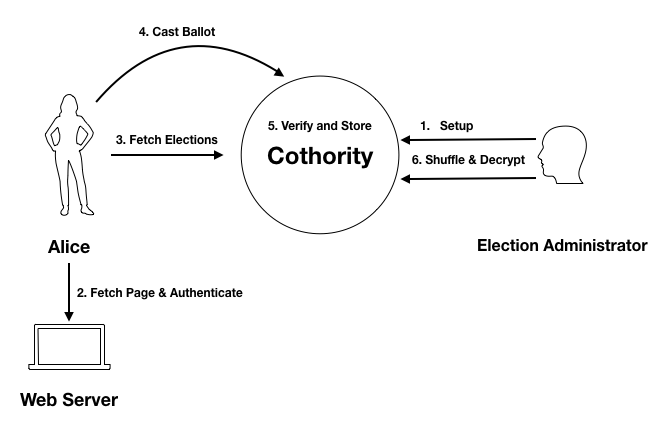
\includegraphics[scale=0.4]{Figures/Overview.png}
    \rule{35em}{0.5pt}
  \caption[Voting Procedure]{Voting Procedure}
  \label{fig:Voting Procedure}
\end{figure}

\begin{enumerate}
\item An election administrator sets up an election with a list of candidates and the users allowed to participate in the election. For this example, let's assume Alice is allowed to vote in one of the elections. Setting up an election happens in a distributed manner with each participating server generating a secret. An aggregate public key is generated using these secrets and it may be used to encrypt messages on client side.
\item Alice visits the frontend client using a browser. The client checks for the presence of a signature in the browser's localStorage \cite{localStorage}, verifying her identity or redirects Alice to an authentication endpoint in its absence.
\item After successful authentication, Alice can see all the elections she is eligible to participate in.
\item Alice may cast as many ballots as she wishes for each election she is allowed to participate in. The ballot is encrypted in the browser before being sent to the backend for storage.
\item Alice's encrypted ballot is then published in a distributed ledger which is accessible to everyone.
\item After the election ends, the election administrator may initiate mixing of all ballots, where the last cast ballot by each user is taken in account and shuffled by a threshold number of participating nodes in the election, one node at a time. The shuffle is stored in the distributed ledger only if a threshold number of nodes can verify its integrity.
\item The last shuffle is then decrypted by each participating node using its share of the secret.
\item Alice or any external auditor may then see the final tally of votes by reconstructing the decryption shares of a threshold number of nodes and counting the decrypted ballots.
\end{enumerate}

It is important to note that the evoting system only encrypts the user's ballots but not their identity. It is therefore possible to ensure if a user voted or not (recorded-as-cast) and the encryption ensures no one can ascertain which candidate(s) the user voted for. The current implementation however does not allow the voter to ensure if their vote is cast-as-intended.

Having introduced the system in brief, we now turn our attention to the system architecture and implementation details
% Chapter Template

\chapter{System Design and Architecture} % Main chapter title

\label{Chapter2} % Change X to a consecutive number; for referencing this chapter elsewhere, use \ref{ChapterX}

\lhead{Chapter 2. \emph{System Design and Architecture}} % Change X to a consecutive number; this is for the header on each page - perhaps a shortened title

%----------------------------------------------------------------------------------------
%	SECTION 1
%----------------------------------------------------------------------------------------

\section{Election Data Structure}

\subsection{Skipchains}

The evoting system makes extensive use of a tamper proof blockchain-like data structure called Skipchains \cite{skipchains}. An amalgamation of blockchain and skiplists, Skipchains allow clients to traverse forward and backwards in a linear data structure using multi hop links in logarithmic time with respect to the length of the chain. As in blockchains, the backward links are cryptographic hashes of the previous blocks. However, the forward links are collective cryptographic signatures of future blocks and are added once the future block is stored. Each additional cosignature on a forward link represents the fact that a witness (a node) examined the block and agrees it follows the verification rules of the evoting system.

The evoting state is maintained in the skipchain with the state being the concatenation of data in all blocks of the skipchain. The subsections below elaborate how the data is actually stored and represented in the skipchain.

\begin{figure}[ht]
  \centering
    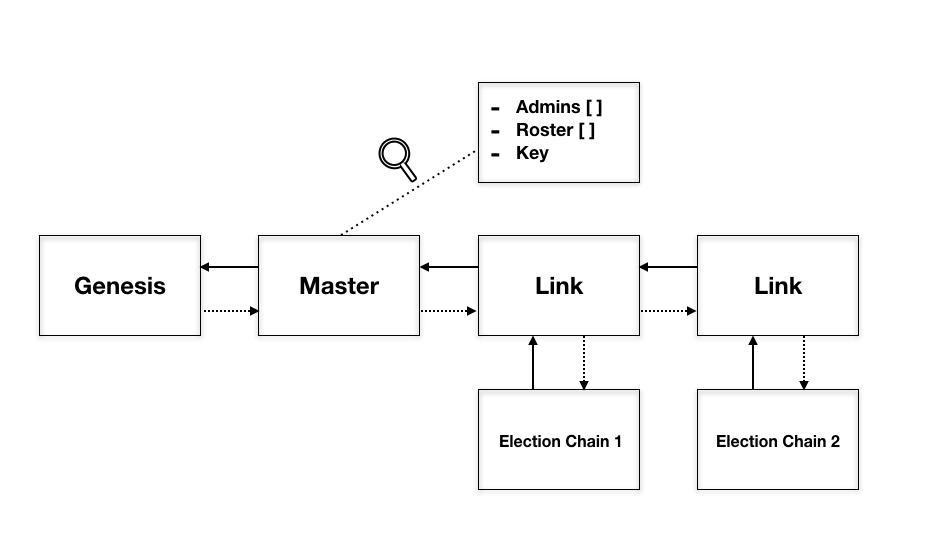
\includegraphics[scale=0.4]{Figures/MasterSkipchain.png}
    \rule{35em}{0.5pt}
  \caption[Master Skipchain]{Master Skipchain}
  \label{fig:MasterSkipchain}
\end{figure}

\subsection{Master Skipchain}

The evoting service is built to support multiple independent elections from the ground up. The global configuration common to a set of elections, and references to those elections themselves are stored in a Skipchain called the Master Skipchain.

Figure \ref{fig:MasterSkipchain} shows an example of a Master Skipchain. The first block, called the genesis block, is empty and contains no data. The next block, called the Master Block contains the following configuration info:

\begin{itemize}
\item Admins: a list of unique 6 digit identifiers for denoting election administrators who may create new elections and finalise them. These identifiers, called \textit{SCIPER}s are used to identify every person across EPFL. 
\item Nodes: a list of servers, called conodes which will participate in the election process.
\item Key: an Ed25519 Public Key used to \hyperref[sec:auth]{verify user authentication signature}.
\end{itemize}

The remaining blocks, called the Link blocks are references to Election Skipchains described in the next subsection. It should be noted that the configuration in the master skipchain may change over time with the addition of new Master blocks. The configuration defined in the latest Master Skipblock wins.

\subsection{Election Skipchain}

All information associated with a particular election is stored in a sidechain, called the Election Skipchain. The Master Skipchain stores a reference to the genesis block of this sidechain in Link Skipblocks.

\begin{figure}[ht]
  \centering
    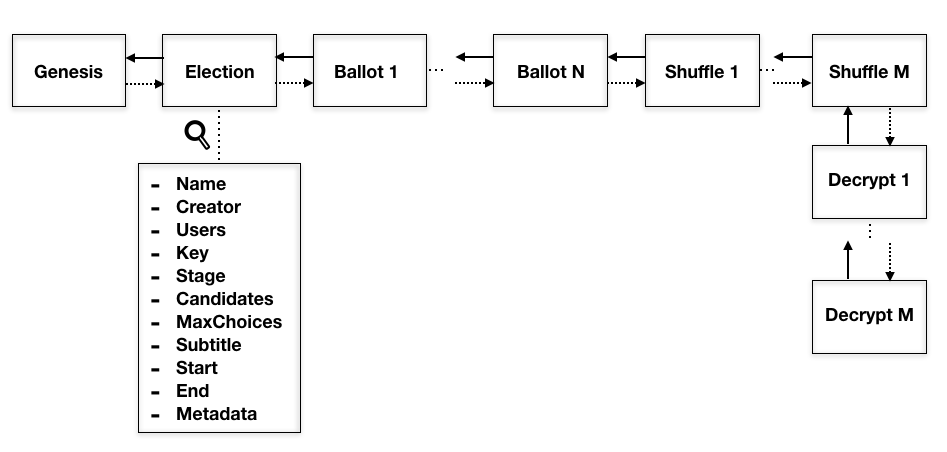
\includegraphics[scale=0.4]{Figures/ElectionSkipchain.png}
    \rule{35em}{0.5pt}
  \caption[Election Skipchain]{Election Skipchain}
  \label{fig:ElectionSkipchain}
\end{figure}

As depicted in Figure \ref{fig:ElectionSkipchain}, the Election Skipchain contains an Election block which stores information associated with the specific election. It contains the following configuration values:

\begin{itemize}
\item Name: Election Title with support for translations in different languages.
\item Creator: Identifier of the administrator who created the election.
\item Users: list of identifiers of users who may vote in this election.
\item Election Public Key: an aggregate public key generated using the DKG Protocol \cite{dkg}, which is used to \hyperref[sec:dkg]{encrypt the ballots}.
\item Stage: the current status of election determined at run time. It may be Running i.e. users may cast their vote, Shuffled i.e. the ballots have been mixed or Decrypted i.e. the ballots have been decrypted by participating nodes using their share of the secret key.
\item Subtitle: Election Subtitle with support for translations in different languages
\item Start: Timestamp of the election start.
\item End: Timestamp of the election end.
\item Metadata: other keys which store metadata related to the election, including the department name, contact person details etc.
\end{itemize}

After the Election Block, the election skipchain consists of a series of Ballot blocks which are stored whenever a user casts a vote. The contents of the Ballot Block include an encrypted ElGamal Ciphertext using the Election Public Key described above.  The encryption algorithm proceeds as follows:

\begin{enumerate}
  \item When a user, say Alice, wants to cast her ballot, the frontend client first encodes the ballot. Each candidate's \textit{SCIPER} is encoded using 3 bytes and upto 9 such \textit{SCIPER}s may be encoded in a ballot. Since the point size is 32 bytes, the remaining bytes are randomly filled such that the resulting 32 byte buffer is a valid point $M$ on the Edwards form of Curve 25519 \cite{ed25519}.
  \item The client then selects a random value \( r \in \mathbb{Z}_{n} \) and computes \( u = rG \) and \( v = M + rY \) where $Y$ is the Election Public Key.
  \item The client then sends the pair \( (u, v) \) to the server for storage in the skipchain.
\end{enumerate}

The Ballot Block also contains an identifier for the user who cast the vote. Since the evoting system allows a user to cast multiple ballots, this field is used to determine the last cast ballot for every user before performing the first shuffle. This design can also be used to send a reminder to users who haven't cast their vote yet.

Once the election is finalised, the election administrator may initiate the shuffle and decrypt protocol which result in the addition of Shuffle and Decrypt blocks in the skipchain. Each shuffle block contains a permutation of last cast ballot by every user which participated in the election and a verifiable proof of the mix which is verified by a threshold number of nodes before the block is stored in the skipchain. A threshold number of participating nodes then add their decryption share to the skipchain in the form of Decrypt blocks. These decryptions are performed on the ballots contained in the last shuffle block in the skipchain.

\section{Architecture}

\begin{figure}[ht]
  \centering
    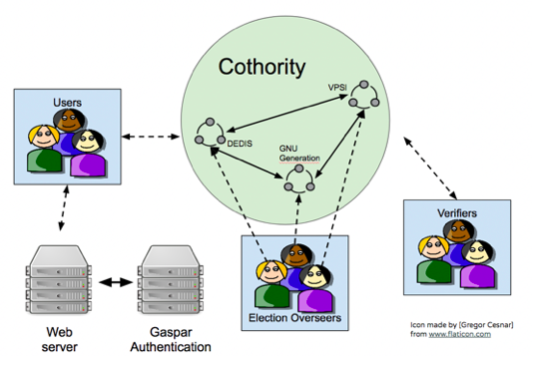
\includegraphics[scale=0.6]{Figures/Architecture.png}
    \rule{35em}{0.5pt}
  \caption[Architecture]{Architecture}
  \label{fig:Architecture}
  \source{Linus Gasser}
\end{figure}

The implementation can be divided into three different components

\begin{enumerate}
  \item A web server that serves static HTML and Javascript files that make up the frontend client.
  \item A web server that acts as an intermediary to authenticate a user against EPFL’s authentication system.
  \item A set of servers, called a \textit{cothority}, with each individual server called a \textit{conode}, which are responsible for handling various protocols associated with the election in a distributed manner.
\end{enumerate}

\subsection{Frontend Webserver}
The frontend server is responsible for serving static HTML and Javascript files to the client. This can be done using any appropriate web server like Nginx. The frontend client configuration contains a reference to the Hash of the Master Skipchain and is used to fetch the list of all elections a user may participate in.

\subsection{Authentication Server}
\label{sec:auth}
The authentication server is a Node.js webserver that facilitates authentication between the user and Tequila, EPFL’s authentication service \cite{tequila}. Tequila allows users to authenticate with the following protocol

\begin{enumerate}
  \item The authentication server sends a POST request to Tequila with the service’s name, redirection URL and requested parameters as the payload. Tequila then replies with a \textit{urlaccess} token.
  \item The authentication server then redirects the user to Tequila. The \textit{urlaccess} token retrieved before is appended as a query parameter to the GET request
  \item Tequila verifies the user details on submission and redirects the user to the redirection URL for the specified \textit{urlaccess} token irrespective of whether the authentication succeeds or not
  \item The authentication server must then send another POST request to Tequila with the \textit{urlaccess} token as a payload. Tequila replies with the user details and parameters requested in the initial request if the authentication was successful or an error is returned otherwise.
\end{enumerate}

It should be noted that as of now Tequila allows verifying the \textit{urlaccess} token mentioned in the last step of the protocol only once. Any further attempt to validate results in an error being returned. This is a limitation in the current design of the evoting service with the authentication server being a single point of failure. On confirmation of successful authentication of the user from Tequila, the authentication server generates a Schnorr signature which is stored in the browser’s localStorage \cite{localStorage}. This signature is used to verify all transactions as described in the next subsection about Cothority.

\subsection{Cothority}

A collective authority (cothority) \cite{cothority} is a set of nodes that witness a particular transaction in a Skipchain and a threshold number of nodes collectively authorise it to be stored. The framework is a research project at the DEDIS laboratory at EPFL, allowing easy deployment of decentralised and distributed services and protocols. The conodes participating in the election run the evoting and skipchain service for orchestrating the elections and storing the data in skipchains respectively.

The skipchain service in the .

\section{Protocols}

The evoting system runs protocols at different stages of the election process to perform operations in a distributed manner. The cothority framework helps in the implementation and testing of these distributed protocols.

\subsection{Consensus Protocol (BFTCoSi)}

The skipchain service in cothority implements a byzantine fault tolerant consensus protocol, called BFTCosi \cite{bftcosi} . BFTCosi is based on the Practical Byzantine Fault Tolerance (PBFT) \cite{pbft} algorithm and uses CoSi \cite{cosi}, a collective signing protocol to aggregate thousands of signatures, to scale itself to thousands of nodes. In particular, BFTCoSi uses CoSi's signing rounds to ensure PBFT's \textit{prepare} and \textit{commit} phase scale to thousands of nodes.

During the execution of the consensus protocol, all nodes in the election roster run a custom verifier function to verify the correctness of the data being stored in the skipchain. All transactions that write data to the skipchain have user identity verification as a part of the verification function. This user identification involves validating the  Schnorr signature of the concatenation of user's identifier and the Master Skipchain's Genesis Block Hash against the Authentication Server's public key which is stored in the Master Skipchain's Master Block.

\subsection{Distributed Key Generation (DKG)}
\label{sec:dkg}
The cothority framework contains an implementation of the Distributed Key Generation (DKG) protocol by Gennaro et. al. \cite{dkg}. The DKG protocol results in the creation of an aggregate public key, and at the same time ensures that the participating nodes hold a share of the secret key and the full secret key is never assembled.

The protocol begins with each node $N_i$ calculating a secret share $s_i$. This is followed by a series of message exchanges that removes potentially malicious nodes and results in a set of qualified nodes \textit{QUAL}. The aggregate secret $x$ is the sum of all the individual secrets of qualified nodes
$x = \sum_{i \in \textit{QUAL}}s_i$. The corresponding public key can be calculated as \(y = gx = g\sum_{i \in \textit{QUAL}}s_i \). The DKG protocol is executed whenever an election administrator requests a new election to be created. Every participating node generates its secret and the aggregate public key is stored in the newly created election skipchain along with other Election Metadata. It is this public key which is used by the frontend client to encrypt the user ballots. The protocol is initialised with a threshold that requires at least \( \lfloor\dfrac{2n}{3}\rfloor + 1 \) nodes to reconstruct the decryptions later where $n$ is the total number of nodes in the roster. The threshold follows from the requirement of having a 2/3rds quorum during the execution of BFTCoSi to store a skipblock.

\subsection{Shuffle}

Once the election ends, the election creator may initiate the shuffle protocol which re-encrypts, permutes and appends the result on the election skipchain providing a proof of the shuffle. The shuffle protocol proceeds as follows:

\begin{enumerate}
  \item The protocol begins with the leader node being contacted by the client to initiate the shuffle. The leader first checks the presence of a threshold number of shuffles already in the skipchain and exits if so.
  \item In the presence of shuffle blocks lesser than the threshold number required, the leader prepares a list of servers which may participate in this instance of the shuffle, excluding the ones that participated before.
  \item In the first attempt at generating the shuffle, the leader iterates through the election skipchain, finding the last ballot cast by each user and appending it to a list. This list is then passed on as an input to the Neff Shuffle function. On the other hand, other attempts at shuffle rely on the last shuffle that is stored in the skipchain and use it as the input to the Neff Shuffle function.
  \item The Neff Shuffle function then permutes the ballots and outputs a permuted list of ballots and a corresponding proof, containing a vector of Scalars that may be used to verify the shuffle \cite{neff}. The node which created the permutation requests the storage of the shuffle which must be ratified by a threshold of participating conodes in the election. The node also signs its public key and stores it in the skipblock, which is then verified by all the participating nodes during the execution of the verification function.
  \item On receiving a request to store the shuffle block, the  participating nodes verify the identity of the node which proposed the shuffle by checking the signature of the public key included in the transaction. They then ensure that the election skipchain does not already have a threshold number of shuffle blocks and the node which has proposed the given shuffle has not stored a shuffle previously. The nodes then run the Neff Shuffle proof verifying the integrity of the shuffle. If all these checks are ratified by a threshold number of participating nodes the shuffle is stored in the skipchain
  \item The proposer then requests the next server in the list to repeat the shuffle until we get a threshold number of shuffles in the skipchain or the protocol times out.
\end{enumerate}

It should be noted that the shuffle protocol is resilient to failures due to non-availability of nodes and timeouts. At every attempt, the protocol tries to pick up from the point where it was abandoned.

\subsection{Decrypt}

The decrypt protocol is used to store a threshold number of decryption shares by the participating nodes. The protocol proceeds as follows:

\begin{enumerate}
  \item The protocol begins with the leader node being contacted by the client to initiate the decryption. The leader first checks the presence of a threshold number of decryptions already in the skipchain and exits if so.
  \item In the presence of decryptions lesser than the threshold number required, the leader prepares a list of servers which may participate in this instance of the decrypt protocol, excluding the ones that participated before.
  \item The leader then sends a broadcast to the whitelisted servers and prompts them to add their decryption share of the last shuffle stored in the skipchain using their share of the private secret generated during the DKG protocol.
  \item Each node sends its decryption share to the skipchain. The participating nodes run the verification function which checks if the election skipchain has threshold number of shuffles in place, verifies the identity of the proposing node by checking the signature of its public key included in the transaction and checks if the node has not stored its decryption share before.
  \item If all the checks pass, the decryption is stored on the skipchain. The node then sends a reply back to the leader indicating success or failure.
  \item The leader maintains a count of successful decryption shares and ends the protocol as soon as a threshold number of success messages are received.
 \end{enumerate}
 
 Like the shuffle protocol, the decrypt protocol is also resilient to failure due to non-availability of nodes and timeouts. Every reinitialisation of the protocol results in an attempt to pick up from the previous failed attempt.

%% Chapter Template

\chapter{Implementation} % Main chapter title

\label{Chapter3} % Change X to a consecutive number; for referencing this chapter elsewhere, use \ref{ChapterX}

\lhead{Chapter 3. \emph{Implementation}} % Change X to a consecutive number; this is for the header on each page - perhaps a shortened title

\section{Backend}

The backend for the evoting implementation makes extensive use of the Cothority framework and as such Go was the natural language of choice for implementing it. The project builds on Andrea Caforio's Master Project work and is split across different packages.

\begin{itemize}
  \item \textbf{struct}: contains definitions of all messages used to interact with the backend using protocol buffers.
  \item \textbf{evoting-admin}: contains an administrative CLI application that is used to set up the Master Skipchain for the election.
  \item \textbf{lib}: contains all library methods and definitions for the evoting application including definitions for transaction structure, methods for storing data on the skipchain using the local skipchain service and over websockets, methods for performing ElGamal encryption, decryption, proving a neff shuffle and utility methods for different operations on the skipchain
  \item \textbf{protocol}: contains implementation of the DKG, Shuffle and Decrypt Protocols as described before.
  \item \textbf{service}: source for the evoting service which receives messages from the frontend client over protocol buffers and performs operations on the skipchain depending on the message type.
\end{itemize}

\section{Frontend}

The frontend client for this project is built using Vue.js \cite{vuejs}. Vue helps in rapid development of the user interface by allowing the composition of reusable components. It also allows efficient DOM updates by leveraging diffing in a Virtual DOM first and syncing only the required changes in the actual DOM.

Since the evoting sytem may be used on mobile devices as well, it was imperative to ensure the frontend is responsive for different screen sizes. In order to have a clean and modern UI, we leverage Vuetify \cite{vuetify}, a UI toolkit for Vue.js.

The routing between different pages of the application is handled using VueRouter \cite{vuerouter}, a routing module for Vue.js. We also use Vuex \cite{vuex} to manage states of different components, cache API responses in memory and in localStorage. The frontend is translated in English, French, German and Italian and uses vue-i18n \cite{vuei18n} for managing the same.

\subsection{KyberJS}
A critical part of voting process is to encrypt the ballots before storing them in the blockchain. While there is some support for cryptographic operations in browsers using javascript with the WebCrypto API \cite{webcrypto}, and in a Node.js environment using the Crypto API \cite{nodecrypto}, they are still in nascent stages and don't support Elliptic Curves we depend on (Ed25519) as of now. Since Javascript provides a unique opportunity to be used in browsers, server side and in native mobile applications (using frameworks like Nativescript \cite{nativescript} and ReactNative \cite{reactnative}), we built a wrapper around a library \cite{elliptic} providing Elliptic Curve Cryptography primitives like \emph{Point} and \emph{Scalar} operations in a finite prime field. The wrapper, called \textit{KyberJS} \cite{kyberjs} adopts an interface similar to its Go equivalent authored by the DEDIS Lab \cite{kyber}. This allows us to leverage a familiar API across browsers, servers and mobile targets and implement new signature and encryption schemes with ease.

\subsection{CothorityJS}
As noted earlier, the set of conodes allow communication over Websockets using Protobufs to encode messages back and forth. In order to facilitate communication between any javascript client and conodes, we built a javascript library, called CothorityJS \cite{cothorityjs}. This library exposes protobuf communication to all the services supported on conodes, (with support for adding new protobuf messages with ease) using a Promise API familiar to javascript developers.
%% Chapter Template

\chapter{Experiments} % Main chapter title

\label{Chapter4} % Change X to a consecutive number; for referencing this chapter elsewhere, use \ref{ChapterX}

\lhead{Chapter 4. \emph{Experiments}} % Change X to a consecutive number; this is for the header on each page - perhaps a shortened title

\section{Setup}

In order to see how the evoting service performs under load, we wanted to setup a set of nodes and simulate elections under different load. Since communication between the frontend and cothority happens over Websockets, a key requirement for the load testing framework was support for websockets. We chose Artillery \cite{artillery}, an extensible open source load testing framework written in Javascript. Artillery's extensibility allows us to write a custom \textit{engine} for it - \textit{artillery-engine-cothority} \cite{artillery-engine-cothority} which allows us to define load test scenarios that can use CothorityJS under the hood to communicate with the conodes.

\begin{figure}[htpb]
  \centering
    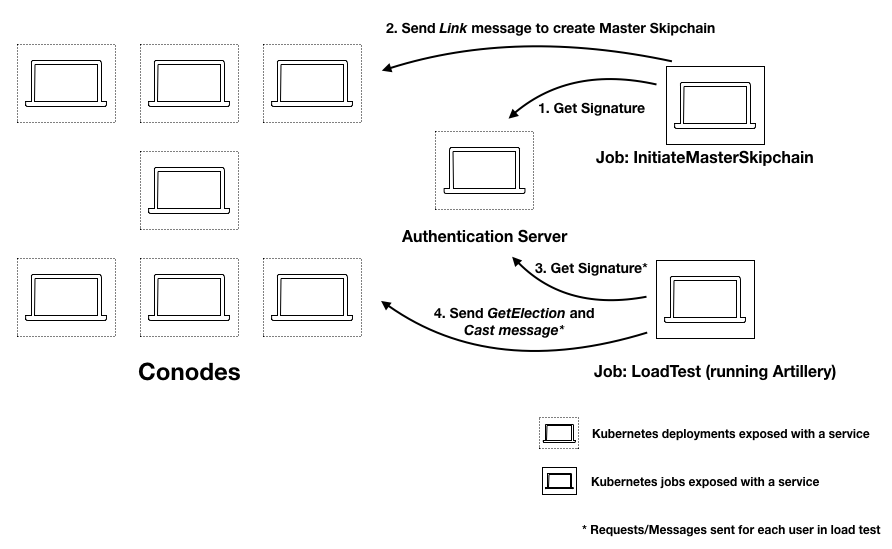
\includegraphics[scale=0.4]{Figures/Kubernetes.png}
    \rule{35em}{0.5pt}
  \caption[Loadtesting]{Loadtesting using Kubernetes and Artillery}
  \label{fig:Loadtesting}
\end{figure}


Next, to simulate our load tests, we used a Kubernetes Cluster provided by the IC Department at EPFL to orchestrate a set of Docker containers running the conodes, the authentication server and the load testing scripts. The end result is an easily configurable setup that allows load testing the evoting service at different transaction rates and different number of conodes. For our experiments, a transaction consists of sending a \textit{GetElection} message (to fetch the list of elections), followed by a \textit{Cast} message (to cast a ballot). This simulates the operations a user would do to cast their vote. The simulations were run with 7 conodes, each running in its own Kubernetes deployment at 2, 3 and 5 transactions per second.

\section{Optimisations}

Initial efforts to load test the evoting service lead to frequent timeouts and scaling issues while trying to fetch the list of elections or cast a ballot. As noted before, the evoting service uses skipchains to persist the transactions. Every block that is to be stored in the skipchain must be proposed by a \textit{leader}, which in case of the evoting application, happens to be the first node in the Election Roster. In an effort to allow all conodes to respond to messages sent by the frontend client, the evoting service in every non-leader node contacted the leader node over websockets to store a transaction. This resulted in a large number of network roundtrips which caused frequent timeouts and scaling issues.

An alternative to the above was to ensure that the frontend client may only communicate with the \textit{leader} which may propose a block using its local skipchain service and propagate it to other non-leader conodes. We therefore save on the network roundtrips in the previous scenario without adding new complexities to the system.

\section{Statistics}

\begin{figure}[!h]
\minipage[b]{0.5\textwidth}
    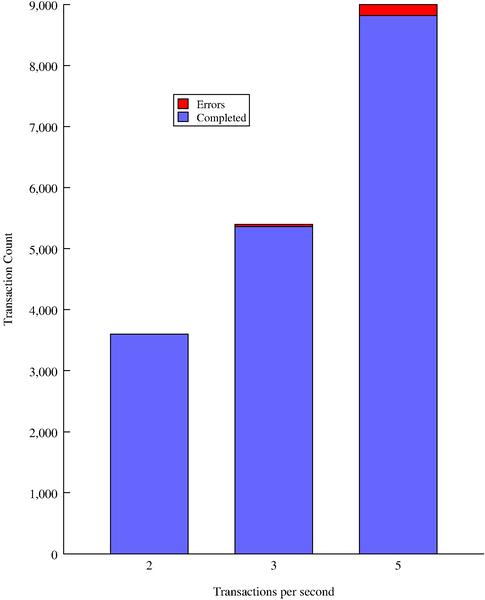
\includegraphics[width=\linewidth]{Figures/ScenarioResponses.png}
  \caption[Scenario Responses]{Scenario Responses}
  \label{fig:ScenarioResponses}
\endminipage\hfill
\minipage[b]{0.5\textwidth}
    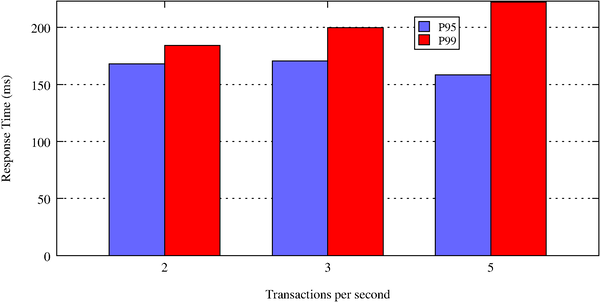
\includegraphics[width=\linewidth]{Figures/AggregateStats.png}
  \caption[Aggregate Statistics]{Aggregate Statistics}
  \label{fig:AggregateStats}
\endminipage\hfill
\end{figure}

After incorporating the optimisations mentioned above, we load tested the evoting service for a duration of 30 minutes at 2, 3 and 5 transactions per second. Figure \ref{fig:ScenarioResponses} shows a plot of the total transaction requests sent, and the proportion that succeeded and failed. We observe that at transaction rates of 2 and 3 TPS, the evoting system manages load fairly well and is quite responsive with 1 and 35 failures respectively. At 5 transactions per second the number of failures increase to 181 out of a total of 9000 transaction attempts.

Figure \ref{fig:AggregateStats} shows the P95 and P99 response times of the service at different loads. As expected response time increases as the service is exposed to a higher transaction rate but it still scales well at a P99 response time of 222.2ms at 5 transactions per second.  In another simulation at 3 transactions per second over 12 hours, the evoting service recorded 118,710 ballots with a P99 response time of 434.3ms.

These statistics indicate that the system should scale well in an Election at EPFL with about 10,000 voters in total. In practice, every department holds its separate election with a smaller list of eligible voters and the voting period being spread over 15 days.

\section{Resilience}

In a distributed architecture it is imperative for the system to be resilient and recover gracefully from node failures. Operations to the skipchain require ratification by \( \lfloor\dfrac{2n}{3}\rfloor + 1 \) nodes following the byzantine consensus requirement. As a result, we've kept the same threshold across all protocols used within evoting. The skipchain service in the conodes is resilient to downtime failures and tries to synchronise itself with the other nodes in the roster when it's available again. The initial implementation of the Shuffle and Decrypt protocols, however, were not resilient to node failures and timeouts and left the election skipchain in an invalid state in case of an error. This occurred because these protocols always assumed they began from a clean state, i.e. no previous attempts were made to Shuffle or Decrypt the election. Recent work on the project was to improve the resilience of these protocols by keeping track of the progress they made before failing, and whitelisting nodes to contact in every run of the protocol, filtering out the ones that have participated before in a previous attempt.
%% Chapter Template

\chapter{Conclusion} % Main chapter title

\label{Chapter5} % Change X to a consecutive number; for referencing this chapter elsewhere, use \ref{ChapterX}

\lhead{Chapter 5. \emph{Conclusion}} % Change X to a consecutive number; this is for the header on each page - perhaps a shortened title

\section{Future Work}
We introduced a distributed, auditable and resilient evoting system that scales well for up to 10,000 users. The system is expected to be used for conducting elections in EPFL in June, 2018. Despite bringing improvements over the current evoting system in place, there is scope to further optimise the evoting system. A projected improvement is to switch from Skipchains to an implementation of Omniledger \cite{omniledger} as the distributed data store. Omniledger adds support for supporting multiple transactions in a block and allows recording malicious attempts to store an invalid block. The latter would be of immense value to an evoting system, since making all attempts to compromise the integrity of an election public would make the system more accountable.

As discussed in section \ref{sec:auth}, the authentication server poses a central point of failure. An improvement would be to use an OAuth like authentication mechanism, supported by Tequila, which would allow each conode to individually verify the \textit{urlaccess} token from the client. While this would incur more network calls, this approach would eliminate the need for an authentication server altogether.

The evoting service can also be extended to support generalised \textit{"Choose M of N"} type of elections without relying on \textit{SCIPER}s or Tequila with suitable alternatives for user identification and authorisation. This will enable it to be used for conducting elections outside EPFL.

\pagebreak

\section{Source Code}
The source code for the conodes can be found at \url{https://github.com/dedis/cothority/tree/master/evoting}. The source code for the frontend, the auth server, artillery-engine-cothority and the load testing scripts can be found at \url{https://github.com/dedis/epfl-evoting}
%\input{Chapters/Chapter6}
%\input{Chapters/Chapter7}

%-------------------------------------------------------------------------------
%	THESIS CONTENT - APPENDICES
%-------------------------------------------------------------------------------

\addtocontents{toc}{\vspace{2em}} % Add a gap in the Contents, for aesthetics

\appendix % Cue to tell LaTeX that the following 'chapters' are Appendices

% Include the appendices of the thesis as separate files from the Appendices
% folder
% Uncomment the lines as you write the Appendices

% Appendix A

\chapter{Protobuf Messages} % Main appendix title

\label{AppendixA} % For referencing this appendix elsewhere, use \ref{AppendixA}

\lhead{Appendix A. \emph{Protobuf Messages}} % This is for the header on each page - perhaps a shortened title

\begin{lstlisting}[caption={Protobuf API Specification}, captionpos=b, language=protobuf2, style=protobuf]
message LookupSciper {
	required string sciper = 1;
}

// LookupSciperReply returns the elements of the vcard from
// https://people.epfl.ch/cgi-bin/people/vCard?id=sciper
message LookupSciperReply {
	required string fullName = 1;
	required string email = 2;
	required string url = 3;
	required string title = 4;
}

message Election {
    map<string, string> name = 1;
    optional uint32 creator = 2;
    repeated uint32 users = 3 [packed=true];
    optional bytes id = 4;
    optional bytes master = 5;
    optional Roster roster = 6;
    optional bytes key = 7;
    optional bytes masterKey = 8;
    optional uint32 stage = 9;
    repeated uint32 candidates = 10 [packed=true];
    required int32 maxChoices = 11;
    map<string, string> subtitle = 12;
    required string moreInfo = 13;
    required sint64 start = 14;
    required sint64 end = 15;
    required string theme = 16;
    required Footer footer = 17;
    optional bytes voted = 18;
}

message Master {
    required bytes id = 1;
    required Roster roster = 2;
    repeated uint32 admins = 3 [packed=true];
    required bytes key = 4;
}

message Footer {
  required string text = 1;
  required string contactTitle = 2;
  required string contactPhone = 3;
  required string contactEmail = 4;
}

message Ballot {
    required uint32 user = 1;
    required bytes alpha = 2;
    required bytes beta = 3;
}

message Ping {
    required uint32 nonce = 1;
}

message Link {
    required string pin = 1;
    required Roster roster = 2;
    required bytes key = 3;
    repeated uint32 admins = 4;
    optional bytes id = 5;
    optional uint32 user = 6;
    optional bytes sig = 7;
}

message LinkReply {
    optional bytes master = 1;
}

message GetElections {
    required uint32 user = 1;
    required bytes master = 2;
    optional uint32 stage = 3;
    required bytes signature = 4;
    optional bool checkVoted = 5;
}

message GetElectionsReply {
    repeated Election elections = 1;
    required bool isAdmin = 2;
    required Master master = 3;
}

message Open{
    required bytes id = 1;
    required Election election = 2;
    required uint32 user = 3;
    required bytes signature = 4;
}

message OpenReply {
    required bytes id = 1;
    required bytes key = 2;
}

message Cast {
    required bytes id = 1;
    required Ballot ballot = 2;
    required uint32 user = 3;
    required bytes signature = 4;
}

message CastReply {
    required bytes id = 1;
}

message Shuffle {
    required bytes id = 1;
    required uint32 user = 2;
    required bytes signature = 3;
}

message ShuffleReply {
}

message Decrypt {
    required bytes id = 1;
    required uint32 user = 2;
    required bytes signature = 3;
}

message DecryptReply {
}


message Reconstruct {
	required bytes id = 1;
}

// ReconstructReply message.
message ReconstructReply {
	repeated bytes points = 1;
}
\end{lstlisting}

%\input{Appendices/AppendixB}
%\input{Appendices/AppendixC}

\addtocontents{toc}{\vspace{2em}} % Add a gap in the Contents, for aesthetics

\backmatter

%-------------------------------------------------------------------------------
%	BIBLIOGRAPHY
%-------------------------------------------------------------------------------

\label{Bibliography}

\lhead{\emph{Bibliography}} % Change the page header to say "Bibliography"

% Use the "unsrtnat" BibTeX style for formatting the Bibliography
\bibliographystyle{ieeetr}

% The references (bibliography) information are stored in the file named
% "Bibliography.bib"
\bibliography{Bibliography}

\end{document}
